\documentclass[preprint,12pt]{elsarticle}
\usepackage[T1]{fontenc}
\usepackage[utf8]{inputenc}
\usepackage{lmodern}
\usepackage{microtype}
\usepackage{graphicx}
\usepackage{float}
\usepackage{xurl}
\usepackage{needspace}
\usepackage{amsmath,amssymb}
\usepackage{booktabs,tabularx,array}
\usepackage{enumitem}
\biboptions{numbers,sort&compress}
\usepackage{xcolor}
\usepackage{tikz}
\usetikzlibrary{positioning,arrows.meta}
\usepackage[colorlinks=true,linkcolor=blue!45!black,citecolor=blue!45!black,urlcolor=blue!45!black,breaklinks=true]{hyperref}
\setlength{\emergencystretch}{2em}
\setlist{nosep,leftmargin=*}
\newcolumntype{Y}{>{\raggedright\arraybackslash}X}
\journal{Journal of Parallel and Distributed Computing}
\makeatletter
\let\ps@pprintTitle\ps@plain
\makeatother
\begin{document}
\begin{frontmatter}
\title{Diagnostic Skill Reuse for Agentic Autotuning\\of Stateful PD-Disaggregated Serving in SGLang}
\author{BoTao Cheng}
\address{Tencent}
\date{}


\begin{abstract}
Prefill--decode (PD) disaggregation exposes configuration choices across phase allocation, parallel execution, batching, and state transfer. Experiments with SGLang on a Kunlunxin P800 pool show that cache reuse, restart procedures, and idle recovery can change the observed behavior of nominally similar deployments. Increasing total throughput can also reduce per-card efficiency or worsen token-generation latency. This paper proposes an experience-constrained diagnostic-skill framework for agentic autotuning. A skill describes its applicable execution state, bounded interventions, competing explanations, expected observations, restoration procedure, and supporting evidence. A language-model controller selects diagnostic actions and parameter families, while a constrained numerical optimizer proposes concrete configurations. Capability and execution contracts govern admissible operations; context changes trigger applicability checks and, when necessary, local replay. The framework distinguishes diagnostic support, process survival, request completion, and service-level attainment. Deployment experiments motivate the design, and an evaluation methodology specifies matched comparisons of numerical search, rule-based control, and agentic skill selection. The research focuses on reducing the total cost of reaching a feasible serving configuration while retaining the ability to revise incorrect experience.

\end{abstract}

\begin{keyword}
LLM serving\sep prefill--decode disaggregation\sep agentic autotuning\sep diagnostic skills\sep resource planning
\end{keyword}
\end{frontmatter}

\section{Introduction}
LLM serving configurations span resource allocation, parallelism, batching, memory management, and communication. Prefill--decode (PD) disaggregation separates prompt processing from subsequent token generation, enabling stage-specific configurations while introducing explicit state transfer. DistServe examines allocation under latency constraints, Splitwise studies phase-specific provisioning, and HexGen-2 considers heterogeneous resources and communication~\cite{distserve2024,splitwise2024,hexgen2025}. Efficient serving therefore requires coordinated decisions across stages and their connections.

Before evaluating another configuration, a tuner must decide which evidence to acquire. A latency increase may reflect prefill pressure, decode admission, cache loading, or state-transfer waiting. These explanations imply different interventions. Searching all parameter families can spend a substantial budget on deployments that do not address the current limitation, while interpreting a plausible explanation without testing it can propagate an incorrect rule.

In preliminary SGLang experiments on P800 accelerators, I observed that cache reuse and execution protocols substantially changed reported throughput and latency. Increasing prefill resources raised total throughput but reduced throughput per card in one configuration comparison. Other trials completed without a process crash yet served only a small fraction of requests successfully. Continuous-load testing and recovery after a long idle interval also exposed different failure paths. These observations motivate explicit checks on the execution state before reusing a tuning decision.

LLM-assisted tuning already combines domain knowledge, numerical optimization, and accumulated experience. GPTuner uses tuning knowledge with optimization; STELLAR accumulates contextual rules; SysInsight links system internals with empirically supported diagnosis~\cite{gptuner2024,stellar2025,sysinsight2026}. This paper focuses on the diagnostic action itself: which controlled observation distinguishes competing stage explanations, and under which conditions can its guidance be reused?

I propose an experience-constrained diagnostic-skill framework with a language-model controller, an authored skill library, a numerical optimizer, and an independent executor and evaluator. Skills specify applicability conditions, permitted interventions, expected observations, and restoration. Historical experience changes search priority rather than permanently excluding legal configurations. When cache state, software, topology, or initialization changes, the controller reviews applicability and can replay the diagnostic.

The paper develops three elements: deployment observations that motivate state-aware tuning; a formulation of evidence acquisition and configuration selection under a common budget; and a constrained skill design with a matched evaluation methodology. The existing experiments use human-selected diagnostic actions executed through tools and skills. Autonomous diagnostic selection is the method to be evaluated, with its value assessed against numerical search, fixed rules, and a tool-using agent.

\section{Background and Related Work}
\subsection{Disaggregated serving and configuration}
PD serving separates the processing of prompts and the generation of subsequent tokens across model replicas. The practical configuration space includes the number of replicas, their parallel strategies, runtime limits, and supported transfer paths. Mooncake organizes service around KV state, and Sarathi-Serve provides an important colocated alternative based on chunked prefill~\cite{mooncake2024,sarathi2024}. A tuned colocated system provides a reference for evaluating PD deployment choices.

SGLang provides a language-model execution system and runtime~\cite{sglang2024}. Its current PD documentation and the SGLang-Kunlun repository provide relevant integration surfaces~\cite{sglangpd,kunlunplugin}. The framework uses a version-specific capability manifest to represent supported parallel strategies, transfer paths, and routing.

Recent preprints also address SLO-aware PD resource counts and coordinated phase/network autoscaling~\cite{pdresources2026,tokenscale2025}. The planner studied here recommends deployments offline and complements online resource-control mechanisms.

Large-scale NVIDIA and Meta studies explore deployment trade-offs with simulation supplemented by empirical measurements~\cite{pragmatic2026,metaconfig2026}. A re-evaluation studies KV transfer media, reuse, and performance--energy implications, while TaiChi unifies aggregation and disaggregation under TTFT/TPOT objectives~\cite{revisiting2026,taichi2025}. The proposed framework focuses on the diagnostic decisions that guide configuration exploration under changing execution state.

\subsection{Numerical and knowledge-guided autotuning}
SCOOT applies constrained Bayesian optimization to inference-engine tuning and handles known and hidden configuration constraints~\cite{scoot2025}. It is a direct algorithmic reference for numerical search. GPTuner extracts tuning knowledge and uses it for knob selection and search-space optimization; $\lambda$-Tune generates complete database configurations and accounts for candidate-evaluation overhead~\cite{gptuner2024,lambdatune2025}. These works motivate comparisons against capable search and knowledge-guided methods rather than against defaults alone.

SLO-Guard studies failure-aware, budget-consistent serving tuning, while ECO combines a structured prior and constrained optimization for disaggregated serving under limited measurements~\cite{sloguard2026,ecotuning2026}. Both are preprints in the cited versions. Their treatment of failures and limited budgets informs the evaluation methodology.

\subsection{Agents, diagnosis, and accumulated knowledge}
STELLAR already supports adaptive analysis, configuration execution, and accumulated rules with tuning contexts. Its rule synthesis also addresses conflicting guidance~\cite{stellar2025}. SysInsight derives hypotheses from code, induces contextual rules from observations, and maintains feedback-based reliability~\cite{sysinsight2026}. StorageXTuner, a preprint, combines agent roles, exploration, and empirically validated insights~\cite{storagextuner2025}. These systems establish context-dependent knowledge and feedback as components of agentic tuning.

The framework uses an explicit action representation for \emph{diagnostic interventions}: what can be changed or observed, which competing stage explanations it can distinguish, and what evidence is required before transferring its guidance. Matched agent and fixed-rule baselines isolate the value of this intervention representation and selection process.

\subsection{Measurement and comparison}
Autotuning comparison must account for elapsed time, stochasticity, and evaluation overhead~\cite{methodology2024}. AutoTuneBench, a recent preprint, studies the reliability of agent-generated serving and kernel measurements~\cite{autotunebench2026}. The evaluation uses independent metric computation and complete elapsed-time and resource accounting.

\section{Deployment Experiments and Motivation}
\label{sec:historical}
\subsection{Experimental setup and metrics}
I deployed DeepSeek V4 Pro using SGLang on servers with dual-socket AMD EPYC 9K84 CPUs, eight Kunlunxin P800 accelerators per server, and RDMA connectivity. The exploratory experiments cover a 32-card 1P1D deployment and a 48-card 2P1D deployment. A prefill replica uses two pipeline stages with TP8 per stage; the decode configuration uses TP16, EP16, and DP8. The workload consists of sessions with prefix reuse, evaluated under fixed client concurrency. The tested concurrency levels include 64, 88, 96, and 128.

The measurements distinguish prefill TPM, decode TPM, total TPM, per-card TPM, TTFT, end-to-end latency, TPOT, cache hit rate, and request completion. Total TPM is the sum of prefill and decode TPM and includes cache-hit tokens. It measures the logical token workload served, rather than only newly computed tokens. TTFT is reported in seconds and TPOT in milliseconds. Process crashes, request failures, and recovery behavior are recorded separately.

The experiments include cold single-pass execution, repeated-session execution, sustained load, parameter changes, and idle recovery. Different protocols expose different execution states. The comparisons below characterize these observed conditions; differences across machine groups, durations, and realized outputs prevent attribution to one configuration factor alone.

\subsection{Cache context and resource trade-offs}
Table~\ref{tab:historical-cache} summarizes three 32-card 1P1D experiments at concurrency 88. After a complete restart and cache clearing, a single pass achieved 6.4401 million total TPM and mean TTFT of 14.9021 seconds. With repeated sessions over two and 24 hours, the observed cache hit rate reached 98.43\% and 99.28\%, respectively, while mean TTFT fell below four seconds. The 24-hour run had 45.29\% higher total TPM than the cold single pass, but mean TPOT increased by 21.53\%.

\begin{table}[htbp]
\centering\small
\begin{tabular}{@{}lrrrr@{}}
\toprule
Execution protocol & \shortstack{Cache hit\\(\%)} & \shortstack{Total TPM\\($10^6$)} & \shortstack{Mean TTFT\\(s)} & \shortstack{Mean TPOT\\(ms)} \\
\midrule
Cold single pass & 89.71 & 6.4401 & 14.9021 & 26.268 \\
2 h repeated sessions & 98.43 & 9.2725 & 3.7549 & 32.431 \\
24 h repeated sessions & 99.28 & 9.3565 & 3.6146 & 31.924 \\
\bottomrule
\end{tabular}
\caption{Observed performance under different cache-reuse and execution protocols on 32-card 1P1D at concurrency 88. The runs differ in duration and realized outputs.}
\label{tab:historical-cache}
\end{table}

These measurements show why the evaluation protocol must accompany a throughput result. Because total TPM includes cache-hit tokens, a higher value does not directly measure additional prefill computation. In the 24-hour run, total TPM was 9.3565 million, while decode TPM was 131154.61, approximately 2185.91 tokens/s. The two quantities describe different aspects of serving capacity. Aggregate cache hits also do not identify the contribution of an individual cache tier.

A second comparison examines resources and latency. At concurrency 96, the 32-card 1P1D deployment produced 5.7713 million total TPM, compared with 7.8373 million for 48-card 2P1D. Total TPM increased by 35.80\%, but TPM per card decreased from 180351.81 to 163276.62, or 9.47\%. Mean TTFT decreased from 23.0321 to 7.7916 seconds, while mean TPOT increased from 24.199 to 29.561 milliseconds (Figure~\ref{fig:historical-resource}). Since the deployments used different resource counts and machine groups, this is an exploratory configuration comparison rather than a fixed-resource scaling result. It motivates explicit resource and service objectives.

\begin{figure}[htbp]
\centering
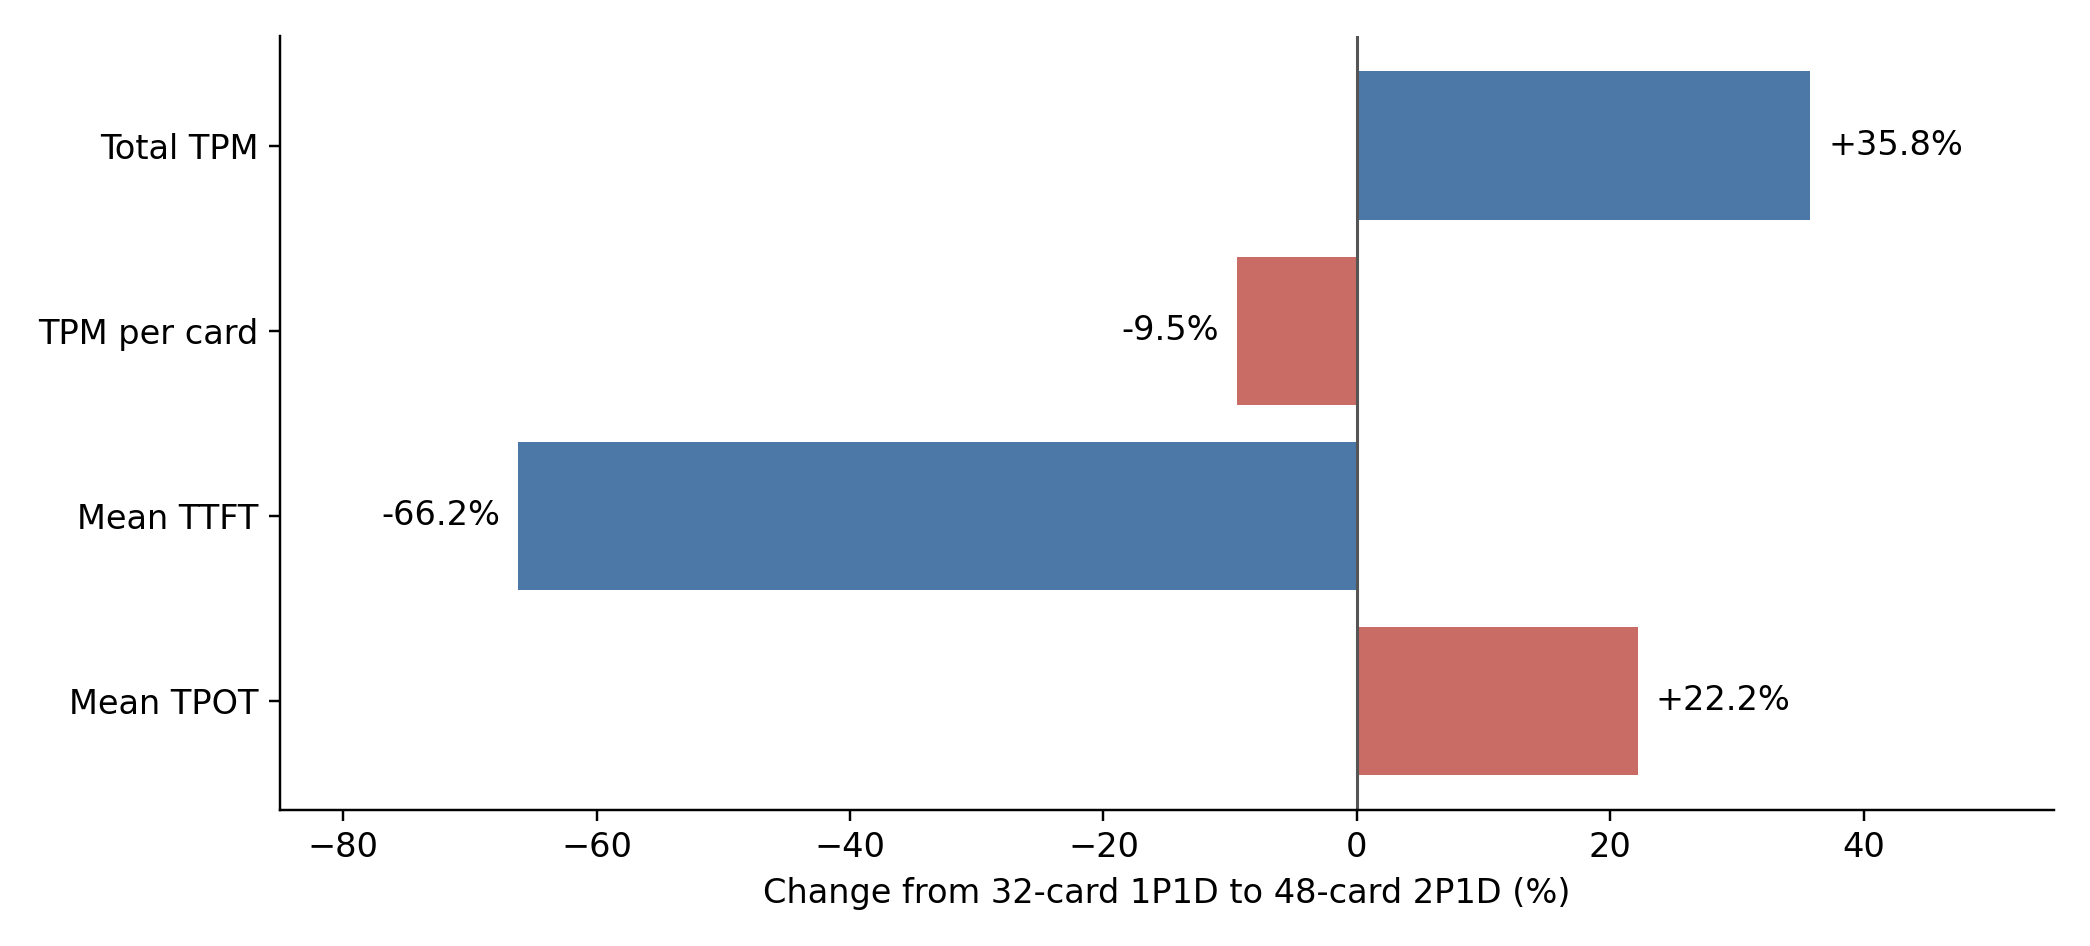
\includegraphics[width=\linewidth]{figures/resource_tradeoff.png}
\caption{Observed resource--performance trade-off between 32-card 1P1D and 48-card 2P1D at concurrency 96. The deployments used different machine groups; the differences are descriptive rather than single-factor effects.}
\label{fig:historical-resource}
\end{figure}

\subsection{Failure diagnosis and execution state}
Restart experiments exposed ambiguity between runtime limits and deployment state. A failure following a prefill parameter change initially suggested a runtime-limit problem; a subsequent trial exposed incompatibility between restarted prefill workers and persistent decode workers. Instability also occurred in a later complete-restart trial. The combined observations support retaining alternative explanations until controlled tests separate them, rather than turning one failed trial into a permanent parameter restriction.

Cache-loading experiments further distinguished process survival from service completion. In one 1800-second trial with asynchronous loading disabled, the processes did not crash, but only 992 of 14461 requests completed successfully (6.86\%). Removing a crash path therefore did not recover usable service. The diagnosis must also consider scheduling progress, cache loading, transfer waiting, and completed requests.

The 24-hour repeated-session test completed 284733 of 284738 requests (99.998244\%) without a recorded process crash. A separate recovery trial after a 5.5-hour idle interval failed; a cold-restart retest did not reproduce that failure. Continuous operation and idle recovery consequently require separate test conditions. The observations identify a state-dependent diagnostic question, without establishing a unique cause for the recovery failure.

In these experiments, I selected the diagnostic interventions and used skills to execute configuration, provisioning, benchmarking, and reporting. This workflow provides the operations and experience for the proposed controller. The skill library encodes the conditions and competing explanations of an intervention; autonomous selection is assessed separately using held-out tasks.

\section{Problem Formulation}
\subsection{Tasks, configurations, and capabilities}
A task is $\tau=(m,w,h,v,\rho,\Delta,\mathcal{S})$, where $m$ identifies the model and fixed precision, $w$ the request process, $h$ the topology, $v$ the software stack, $\rho$ the initialization and state protocol, $\Delta$ the evaluation horizon, and $\mathcal{S}$ the service objectives. The protocol records cache clearing or reuse, deployment generations, idle exposure, session order, and warm-up boundaries. These are controlled conditions, not assumed observable internal state. Workload features include actual input/output length distributions and arrival variability. Maximum output length cannot replace the measured distribution.

A configuration is
\begin{equation}
 c=(n_P,n_D,p_P,p_D,\pi,b_P,b_D,k),
\end{equation}
where $n_P,n_D$ are replica counts, $p_P,p_D$ are supported parallel strategies, $\pi$ maps workers to resources, $b_P,b_D$ are runtime limits, and $k$ contains supported state-transfer settings. The legal set $\mathcal{C}_{\tau}$ follows from the capability manifest, memory feasibility, and resource availability. Model and KV precision remain fixed within a comparison. Counts denote complete replicas, not arbitrary divisions of model weights.

Let $A(c)$ be the number of allocated accelerator cards; whole-node allocation is recorded separately when it determines reclaimable resources. The formulation does not assume equal resource use per replica or that a model fits on a particular number of P800 cards. Structural changes can require redeployment. The first implementation is an offline planner; online elasticity and in-flight migration are outside its initial scope.

\subsection{Service feasibility and objectives}
For request $i$, define
\begin{equation}
 z_i(c)=\mathbf{1}\{\text{complete}_i \land f_i\leq\theta_f
                  \land o_i\leq\theta_o\},
\end{equation}
where $f_i$ is client-observed TTFT and $o_i$ is the request-level mean interval between output tokens. The primary workload will have at least two output tokens. Any shorter completions will be reported separately using a prespecified eligibility policy. Failures, timeouts, and rejected requests remain in the offered-request denominator.

For a fixed arrival cohort of $N$ requests,
\begin{equation}
 \widehat a(c)=\frac{1}{N}\sum_{i=1}^{N}z_i(c).
\end{equation}
For a stable offered arrival rate $\lambda$, $\lambda\widehat a(c)$ is an attained-arrival-rate estimate. This estimate is distinguished from completion-window throughput, with arrival, observation, and drain intervals reported explicitly. Queue stability and a fixed timeout policy are required to prevent short measurement windows from concealing overload. Separate marginal tail objectives do not imply the same joint attainment.

The capacity-planning objective is
\begin{equation}
 \min_{c\in\mathcal{C}_{\tau}} A(c)
 \quad\text{subject to}\quad
 a(c)\geq\alpha,\quad\text{stable queues}.
 \label{eq:capacity}
\end{equation}
The system will return the smallest \emph{measured feasible} configuration it has found, not a certified global optimum. Within an equal-resource stratum, a secondary objective maximizes attained service capacity. A separate tuning objective minimizes the cost of reaching a prespecified feasible performance target. These objectives are reported separately to distinguish resource consumption from latency.

\subsection{Budgeted evidence acquisition}
At step $t$, the controller chooses an action $a_t$ from reading existing evidence, executing a diagnostic skill, evaluating a configuration, or stopping. Its state is $s_t=(\tau,c_t,\mathcal{D}_t,\mathcal{K}_t,\mathcal{H}_t,B_t)$: observations, the skill library, revisable hypotheses, and remaining budget. $\mathcal{H}_t$ need not contain calibrated probabilities. A language model's confidence is not a measurement of bottleneck probability.

Every action has elapsed-time cost $T(a_t)$ and resource cost
\begin{equation}
 C_A(a_t)=\int_{\text{action interval}} A_t(u)\,du.
\end{equation}
Diagnosis, model loading, restarts, warm-up, recovery, and controller inference are charged. Concurrent experiments must satisfy a common resource ceiling or common allocation-time budget, with the selected protocol fixed across methods.

\section{Proposed Method}
\subsection{Stage-aware evidence rather than a fixed latency equation}
The controller uses a stage dependency graph containing client submission, request admission, prefill work, state readiness, transfer, decode admission, and token emission where those events are observable. This graph is a description of the deployed implementation, not a universally additive latency model. Transfer and computation can overlap. The origin and forwarding of the first streamed token are backend-dependent; decode admission or KV transfer must not automatically be charged to TTFT without tracing the actual first-token path.

Evidence records contain event semantics, clock domains, units, sample sizes, and missingness. Cross-node durations require synchronized clocks with characterized error or durations measured within one clock domain. The LLM receives references to these records and structured summaries. An unavailable counter is marked unknown rather than replaced by a plausible estimate. Diagnostic instrumentation is measured separately so that its overhead is not silently attributed to ordinary serving.

\subsection{A diagnostic skill as an executable experiment}
A diagnostic skill is represented by
\begin{equation}
 \sigma=(P,O,H,I,V,F,R,E,G),
\end{equation}
where $P$ specifies applicability; $O$ required observations; $H$ explanations; $I$ a bounded observation or intervention program; $V$ outcomes of support, contradiction, or inconclusive; $F$ parameter families; $R$ restoration; $E$ provenance-linked evidence; and $G$ an externally checked constraint contract. Initial skills are engineering-authored. Prior interventions initialize context-dependent hypotheses and warnings.

A skill separates diagnostic outcomes from tuning rewards. A probe may support a transfer-contention hypothesis without improving end-to-end goodput. Conversely, a configuration may improve the objective while leaving its supposed explanation unresolved. Neither observation automatically validates the other. The record therefore has separate fields for hypothesis evidence, service feasibility, resource use, and objective change.

An initial library will cover prefill pressure, decode capacity or admission pressure, PD allocation imbalance, and transfer--compute interaction. These are alternative explanations and may coexist. Each skill must state what it holds fixed, what it varies, whether it needs redeployment, and what would make its outcome uninterpretable. A temporary change in cache state, precision, offered workload, or total allocation must not be presented as an isolated parameter effect.

\subsection{Experience-constrained skill execution}
The proposed contract separates four checks:
\begin{equation}
 G=(G_{\mathrm{cap}},G_{\mathrm{exec}},G_{\mathrm{eval}},G_{\mathrm{reuse}}).
\end{equation}
Capability checks restrict operations to the deployed manifest. Execution checks require typed parameters, resource reservation, declared intervention scope, restoration, and budget bounds. Evaluation checks preserve model/precision, workload protocol, metric formulas, and SLO denominator. Reuse checks bind guidance to a versioned state context and request observations or replay when needed. Missing preconditions produce explicit unresolved or non-executable outcomes; the LLM must not silently fill them.

\begin{table}[htbp]
\centering\small
\begin{tabularx}{\linewidth}{@{}>{\raggedright\arraybackslash}p{29mm}YY@{}}
\toprule
Contract & Execution condition & Executor behavior \\
\midrule
Capability & Supported backend operations & Reject operations outside the capability manifest \\
Execution/state & Restart-state consistency & Check worker generations; apply the recovery protocol \\
Evaluation & Process and service outcomes & Separate survival, completion, and joint SLO attainment \\
Reuse & Changed execution context & Reassess cache, idle, software, and topology changes \\
\bottomrule
\end{tabularx}
\caption{Constraint contracts for diagnostic skill execution.}
\label{tab:contracts}
\end{table}

All controllers receive the same mandatory legality and measurement checks. The fixed-rule baseline receives identical skills and initial evidence. Otherwise gains might reflect unequal safeguards rather than agent decisions. Historical runtime-limit warnings remain context-local guidance; only independently established capabilities justify hard exclusion from the legal space.

Restart consistency illustrates the distinction. The study can require a coordinated P/D restart for a declared transition, while a backend-certified compatible partial restart remains legal under its manifest. One historical failure is not a universal restart rule. Disabling asynchronous loading is likewise not accepted as an improvement merely because a crash disappears: service feasibility and cost are evaluated separately.

Each invocation records contract decisions, input/context hashes, source runs, expected distinguishing observations, outcome, objective change, restoration, and charged cost. The record distinguishes human-selected interventions from autonomous choices. Later contradictions append their scope and reason while preserving the original observation.

\subsection{Applicability checks and local replay}
Reuse proceeds through three checks. First, an executable compatibility predicate checks the observations and actions needed by the skill. An absent capability rejects the action. A software or model change whose effects are unknown instead makes the skill unvalidated for the new context; it need not make the diagnostic procedure itself illegal.

Second, the controller compares the current context with contexts in the evidence record. Workload and scale features are normalized using a transformation fixed on source tasks. A transparent distance and coverage rule will flag extrapolation. Thresholds will be chosen on source validation tasks and frozen before held-out evaluation. Similarity is only a retrieval aid and is not a correctness guarantee.

Third, stale, insufficient, or out-of-coverage guidance requires local replay of its diagnostic action. A replay can revalidate an expectation, contradict it, or remain inconclusive. The last outcome does not count as a negative result. Evidence is stored by task and context so that failure on one topology does not erase valid observations elsewhere. Revalidation reduces unsupported transfer; it provides no universal guarantee that a skill is useful.

\subsection{Selecting a diagnostic action}
The LLM proposes a bounded list of skill identifiers and attaches evidence references, competing explanations, and predicted distinguishing observations. It produces structured decisions, not an unrestricted script or a self-certified diagnosis. A deterministic checker verifies that each proposal uses available observations and a legal intervention. Duplicate or non-discriminating proposals are returned for revision.

The initial selection policy will prefer reading already collected evidence, followed by a low-cost diagnostic expected to separate unresolved explanations. An experimental candidate score is
\begin{equation}
 Q(d)=\frac{U(d)}{\widehat C(d)+\varepsilon},
\end{equation}
where $U(d)$ estimates discrimination among current explanations and $\widehat C(d)$ estimates cost under the selected accounting protocol. Before a calibrated predictor exists, $U(d)$ will be an explicit ordinal engineering rubric with an ``unknown'' value; the score is ordinal rather than a calibrated information-gain or causal-probability estimate. The rubric, cost estimator, and tie-breaking policy will be fixed before comparison. The value of LLM proposal generation will be evaluated against an identical rule-based selector.

The diagnostic evidence updates a set of supported, contradicted, and unresolved expectations. Multiple bottlenecks are allowed. When the available probes cannot discriminate, the controller falls back to broader numerical exploration. This fallback is important: the design does not assume that every workload admits an inexpensive and correct diagnosis.

\subsection{Guiding numerical search without permanent exclusion}
A supported diagnostic prioritizes a parameter family and suggests legal initialization points. Structural proposals include replica counts and worker placement; within a structure, the numerical optimizer chooses supported runtime values. The first implementation will use one documented constrained optimizer and retain an unmodified version as a baseline.

Skill guidance affects proposal priority, not hard feasibility, except for independently established capability constraints. In particular, a fraction $\epsilon>0$ of proposal opportunities remains available to the full legal space:
\begin{equation}
 q_t(c)=(1-\epsilon)q_t^{\mathrm{guided}}(c)
                 +\epsilon q_t^{\mathrm{global}}(c).
\end{equation}
The proposal distributions and $\epsilon$ will be declared in the implementation specification. Full-space sampling does not prove convergence under a finite budget; its purpose is to limit irreversible exclusion caused by an incorrect diagnosis. A fixed no-improvement rule can trigger a return to diagnosis or increase global exploration, with its extra cost recorded.

An accepted configuration must be measured. A predictor or an agent-generated explanation cannot make an untested configuration the final recommendation. Final evaluation uses a frozen configuration and independent requests; exploratory measurements do not substitute for held-out service validation.

\subsection{Updating evidence and stopping}
Skill records preserve positive, negative, and inconclusive outcomes, context signatures, configuration changes, and raw run identifiers. Empirical support frequencies, if displayed, are conditional on observed interventions and are not interpreted as causal probabilities. The controller retains multiple hypotheses instead of fitting an unrestricted causal model from sparse trials.

Stopping occurs on budget exhaustion, attainment of a prespecified target followed by independent confirmation, or a declared termination rule. An agent may request stopping, but the executor checks the rule. If no feasible configuration is measured, the output reports that outcome and the tested scope. It does not silently relax the SLO or change the model.

\begin{figure}[t]
\centering
\resizebox{\linewidth}{!}{%
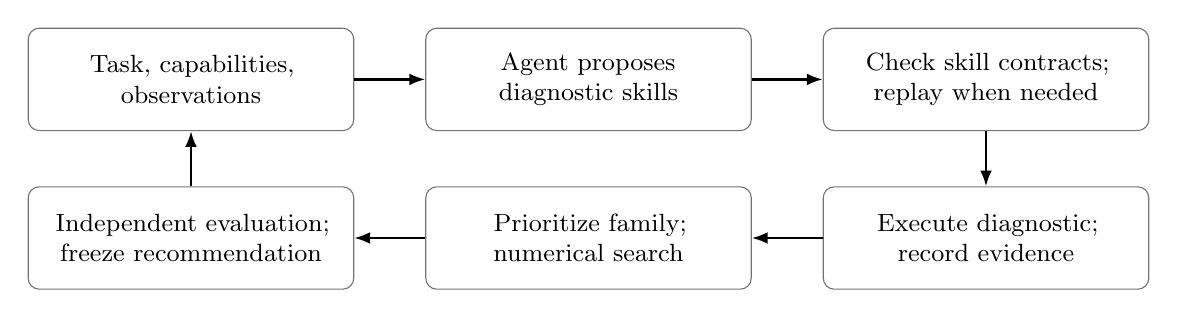
\begin{tikzpicture}[node distance=7mm and 9mm,box/.style={draw=black!55,rounded corners,align=center,font=\small,text width=39mm,minimum height=13mm},arr/.style={-{Latex[length=2mm]},thick}]
\node[box] (state) {Task, capabilities,\\observations};
\node[box,right=of state] (agent) {Agent proposes\\diagnostic skills};
\node[box,right=of agent] (gate) {Check skill contracts;\\replay when needed};
\node[box,below=of gate] (probe) {Execute diagnostic;\\record evidence};
\node[box,left=of probe] (search) {Prioritize family;\\numerical search};
\node[box,left=of search] (eval) {Independent evaluation;\\freeze recommendation};
\draw[arr] (state)--(agent); \draw[arr] (agent)--(gate);
\draw[arr] (gate)--(probe); \draw[arr] (probe)--(search);
\draw[arr] (search)--(eval); \draw[arr] (eval)--(state);
\end{tikzpicture}%
}
\caption{Control flow of the proposed diagnostic-skill framework. Evidence updates retain their source interventions.}
\label{fig:architecture}
\end{figure}

\section{System Design and Algorithm}
\subsection{SGLang and P800 adapter boundary}
The adapter will expose capability discovery, deployment, observation collection, diagnostic execution, benchmark execution, restoration, and configuration freezing. Logical parameters are translated to flags only after checking the deployed version. The controller operates outside the token-generation hot path. It is not proposed as a per-token scheduler.

The capability manifest records model and tokenizer identifiers, weight and KV types, runtime and plugin revisions, attention implementation, parallel configurations, graph and cache modes, transfer backend, and supported routing. CPU, XPU, PCIe, and NIC topology are inventoried instead of inferred from socket count. Capability discovery records device memory, network interfaces, and transport behavior for the active deployment.

Deployment operations carry a resource reservation and restoration plan. Diagnostic probes run on designated experimental resources, and all benchmark parsing and objective computation occur outside agent-editable decisions. The agent can select registered operations, but cannot modify evaluation inputs, metric formulas, or baseline configurations during a comparison. The evaluator remains independent of the controller.

\Needspace{8\baselineskip}
\subsection{Proposed algorithm}
\begin{quote}\small\raggedright
Input: task, legal resources, capability manifest, initial skills, budgets.\\
1. Measure a declared initial configuration; create evidence records.\\
2. While budget remains:\\
\hspace*{1em}a. Retrieve compatible skill candidates and context records.\\
\hspace*{1em}b. Request structured diagnostic proposals from the controller.\\
\hspace*{1em}c. Check contracts and state; read or replay diagnostics.\\
\hspace*{1em}d. Record evidence, provenance, and service outcomes.\\
\hspace*{1em}e. Propose a legal configuration with guided/global search.\\
\hspace*{1em}f. Deploy, warm, measure, restore when required; charge all costs.\\
\hspace*{1em}g. Update the optimizer and context-specific skill records.\\
\hspace*{1em}h. Check the declared stop or return-to-diagnosis rule.\\
3. Freeze and independently validate the best measured feasible candidate.\\
Output: configuration and evidence, or no measured feasible configuration.
\end{quote}
The algorithm defines the proposed autonomous loop. It builds on the existing skill execution workflow and separates diagnostic selection, configuration search, and independent evaluation.

\section{Evaluation Methodology}
\subsection{Research questions}
RQ1 asks whether the method reaches a prespecified feasible target faster than constrained numerical search and an ordinary tool-using agent. RQ2 asks whether diagnostic selection changes useful configuration decisions relative to a fixed-rule controller with identical skills. RQ3 asks whether local replay and applicability checks improve skill transfer to held-out contexts. RQ4 asks how the final recommendations compare in resource use and attained service capacity across deployment scales.

\subsection{Testbed, tasks, and splits}
The evaluation uses the P800 resource pool described in Section~\ref{sec:historical}. Checkpoint and precision are held fixed within a comparison. With 16-card complete replicas and supported routing, the planned resource comparisons include 2P1D versus 1P2D at 48 cards and 3P1D/2P2D/1P3D at 64 cards, alongside 32-card 1P1D. Each layout must pass capability and memory checks. A second model configuration will test generalization where backend support permits.

Workloads cover short-input/short-output, long-input/short-output, short-input/long-output, and mixed-length requests. Open-loop arrivals measure service capacity and queue stability; fixed-concurrency tests provide complementary pressure and mechanism measurements. Cold initialization, repeated reuse, and idle recovery are evaluated separately.

Development experiments supply the initial authored skills. Their context transformations and thresholds are selected on source validation tasks and frozen before held-out model, load, state, or scale tests. Cold-start tuning, tuning with prior experience, and within-task updates are reported separately. All controllers receive matched initial knowledge, legal actions, resource ceilings, and cost accounting.

\subsection{Baselines and component attribution}
\begin{table}[H]
\centering\small
\begin{tabularx}{\linewidth}{@{}>{\raggedright\arraybackslash}p{36mm}YY@{}}
\toprule
Method & Shared conditions & Purpose \\
\midrule
Tuned native serving & Colocated/chunked-prefill and native PD; fixed model and precision & End-to-end engineering reference \\
Constrained optimizer & Same legal space, budgets, and measurement protocol & Benefit beyond numerical search \\
Fixed-rule controller & Same skills, observations, and initial knowledge & Necessity of LLM decisions \\
Tool-using agent & Same model and tools; ordinary feedback and log retrieval & Benefit beyond generic agent orchestration \\
Unconditional skill reuse & Same library; no guidance revalidation; mandatory checks retained & Cost of incorrect transfer \\
Complete proposal & All declared components & Combined effect and overhead \\
\bottomrule
\end{tabularx}
\caption{Controller comparisons and shared evaluation conditions.}
\end{table}

The knowledge-accumulating agent baseline draws on STELLAR and SysInsight. Any adaptation to SGLang uses the same evidence and executor interfaces; comparisons use locally measured results. Ablations will remove active diagnosis, replace skill records with raw-log retrieval, disable applicability replay, and remove global exploration, one mechanism at a time.

\subsection{Metrics, uncertainty, and resource accounting}
Primary metrics are allocation-time and elapsed time to a prespecified target, joint SLO attainment, and final measured resource use at the same offered workload. Secondary metrics include output-token throughput, actual input/output lengths, per-request TTFT/TPOT, token-level inter-token latency, failed configurations, redeployments, and diagnostic actions. P99 results require adequate sample sizes and explicit uncertainty. Diagnostic precision will be reported only for cases with controlled or independently established explanations.

The prospective comparison uses at least three independent repeats of core serving points and multiple controller/search seeds, initially five where affordable. Run order will be randomized or interleaved. Paired comparisons will use the same workload realizations. Requests within one overloaded run are not treated as independent repetitions of the entire tuning process. Unreached targets will be reported as censored outcomes, not dropped when calculating time-to-target.

Thresholds, model selection, search ranges, stopping conditions, the agent prompt, generation settings, and token budgets will be fixed before final evaluation. Agent inference will use separate capacity or have its interference explicitly measured. Parallel searches will share an equal resource ceiling or be compared using an equal allocation-time budget. Offline library construction and online tuning costs will be separated, with amortization reported rather than assumed.

\subsection{Mechanism tests and decision consequences}
The first mechanism test compares isolated transfer, isolated decode, and their controlled concurrent execution when the backend exposes suitable operations. Another compares a stage-capacity recommendation with end-to-end configuration ranking. These tests evaluate whether stage-level estimates distinguish the end-to-end configuration choices.

For each successful diagnostic, the evaluation traces the decision chain: observations, alternatives considered, chosen probe, probe outcome, changed search priority, selected configuration, and independent validation. For an incorrect diagnostic, it reports the wasted cost and whether replay or global exploration recovered. This analysis connects the skill mechanism to a measurable outcome rather than treating explanation quality as a proxy for performance.



\section{Limitations and Threats to Validity}
The deployment experiments characterize one accelerator family and one session workload. Several comparisons change machine groups, execution duration, cache state, or actual output lengths; they therefore motivate hypotheses rather than isolate a unique mechanism. Aggregate timing summaries do not establish tail latency or joint SLO attainment. Request-level traces and independent repeated runs are needed for those measurements.

The proposed agentic controller has not yet undergone matched autonomous tuning experiments. The current observations arise from human-selected interventions and skill execution. They support the skill design but do not establish an advantage over numerical optimization, fixed rules, or existing tuning agents. The evaluation methodology separates those contributions and charges diagnostic and restoration overhead.

Observability and instrumentation also affect validity. Missing stage events can leave competing explanations unresolved, while instrumentation can perturb execution. Cache signatures and thresholds may overfit development tasks. Network variation, co-tenancy, and output-length variability can confound an intervention even when one configuration field changes.

Language-model proposals may omit alternatives or misunderstand parameter semantics. Registered actions, explicit evidence, and independent checks reduce these risks without guaranteeing correct diagnosis. Reduced tuning time and improved final serving capacity remain separate outcomes. The present scope excludes automatic kernel rewriting, precision/quality trade-offs, cross-vendor KV interoperability, and production online migration.

\section{Conclusion}
This paper proposes experience-constrained diagnostic skills for agentic autotuning of SGLang PD serving. P800 deployment experiments motivate three requirements: record execution state with performance, distinguish survival from completed service, and evaluate resource efficiency alongside latency. The framework connects these requirements to bounded interventions, context-dependent reuse, and constrained numerical search. Its central research question is whether selecting and revalidating diagnostic actions reduces the total cost of reaching a feasible configuration. Matched autonomous-controller evaluation remains future work.



{\footnotesize
\interlinepenalty=10000
\setlength{\bibsep}{2pt plus 1pt minus 1pt}
\bibliographystyle{elsarticle-num}
\bibliography{references}
}
\end{document}
